\documentclass[12pt]{report}
\usepackage[utf8]{inputenc}
\usepackage[russian]{babel}
%\usepackage[14pt]{extsizes}
\usepackage{listings}

% Для листинга кода:
\lstset{ %
language=python,                 % выбор языка для подсветки (здесь это С)
basicstyle=\small\sffamily, % размер и начертание шрифта для подсветки кода
numbers=left,               % где поставить нумерацию строк (слева\справа)
numberstyle=\tiny,           % размер шрифта для номеров строк
stepnumber=1,                   % размер шага между двумя номерами строк
numbersep=5pt,                % как далеко отстоят номера строк от подсвечиваемого кода
showspaces=false,            % показывать или нет пробелы специальными отступами
showstringspaces=false,      % показывать или нет пробелы в строках
showtabs=false,             % показывать или нет табуляцию в строках
frame=single,              % рисовать рамку вокруг кода
tabsize=2,                 % размер табуляции по умолчанию равен 2 пробелам
captionpos=t,              % позиция заголовка вверху [t] или внизу [b] 
breaklines=true,           % автоматически переносить строки (да\нет)
breakatwhitespace=false, % переносить строки только если есть пробел
escapeinside={\#*}{*)}   % если нужно добавить комментарии в коде
}

% Для измененных титулов глав:
\usepackage{titlesec, blindtext, color} % подключаем нужные пакеты
\definecolor{gray75}{gray}{0.75} % определяем цвет
\newcommand{\hsp}{\hspace{20pt}} % длина линии в 20pt
% titleformat определяет стиль
\titleformat{\chapter}[hang]{\Huge\bfseries}{\thechapter\hsp\textcolor{gray75}{|}\hsp}{0pt}{\Huge\bfseries}


% plot
\usepackage{pgfplots}
\usepackage{filecontents}
\usetikzlibrary{datavisualization}
\usetikzlibrary{datavisualization.formats.functions}

\begin{document}
 
%\def\chaptername{} % убирает "Глава"
\begin{titlepage}
	\centering
	{\scshape\LARGE МГТУ им. Баумана \par}
	\vspace{3cm}
	{\scshape\Large Лабораторная работа №5\par}
	\vspace{0.5cm}	
	{\scshape\Large По курсу: "Анализ алгоритмов"\par}
	\vspace{1.5cm}
	{\huge\bfseries Конвейер\par}
	\vspace{2cm}
	\Large Работу выполнил: студент группы ИУ7-53Б Наместник Анастасия\par
	\vspace{0.5cm}
	\LargeПреподаватели:  Волкова Л.Л., Строганов Ю.В.\par

	\vfill
	\large \textit {Москва, 2020} \par
\end{titlepage}

\tableofcontents

\newpage
\chapter*{Введение}
\addcontentsline{toc}{chapter}{Введение}

	\textbf{Конвейер} - это способ организации вычислений, используемый в современных процессорах и контроллерах с целью повышения их производительности (увеличения числа инструкций, выполняемых в единицу времени — эксплуатация параллелизма на уровне инструкций), технология, используемая при разработке компьютеров и других цифровых электронных устройств \cite{Conveyer}.
В рамках этой лабораторной работы будут рассмотрены три операции на массиве, которые будут последовательно обрабатываться на 3х конвейерных лентах. Каждая задача
будет последовательно проходить три этапа обработки. Организация многопоточного режима программирования позволит достигнуть максимальной эффективности выполнения программы.

	Целью данной лабораторной работы является изучение и реализация конвейера для выполнения элементарных операций на массиве, а также сравнительный анализ затрачиваемых временных ресурсов при параллельной и однопоточной реализаций одного и того же алгоритма.

В данной лабораторной работе требуется решить четыре задачи.
\begin{enumerate}
\item Изучить основы конвейерной обработки данных.
\item  Получить практические навыки конвейерной обработки данных.
\item Программно реализовать три алгоритма.
\item Сделать сравнительный анализ по затрачиваемым ресурсам (времени) компьютера.
\end{enumerate}


\chapter{Аналитическая часть}
 
 В данной лабораторной работе метод конвейерной обработки данных будет применен к следующим трем стандартным операциям на матрице.
\begin{enumerate}
\item Поиск минимума.
\item Поиск максимума.
\item Подсчет количества элементов.
\end{enumerate}
  Ниже будут представлены теоретические сведения, необходимые для программной реализации этой задачи.
 
 \section{Поиск максимума/минимаума} 
  В лабораторной работе будет рассмотрен простейший и быстрый алгоритм поиска максимального и минимального элементов массива. Следует пояснить, что под быстротой алгоритма будет подразумеваться его асимптотическая сложность, а не физическое время выполнения. В действительности, единственный способ точно найти самое большое или самое маленькое число в случайном массиве будет перебор каждого числа в поисках максимума или минимума. Поэтому сложность такого алгоритма – O(N). Они называются линейными \cite{MaxMin}.
  
\section{Параллельное программирование}

Параллельное программирование - это техника программирования, которая использует преимущества многоядерных или многопроцессорных компьютеров и является подмножеством более широкого понятия многопоточности. Таким образом, параллельные вычисления - способ организации компьютерных вычислений, при котором программы разрабатываются, как набор взаимодействующих вычислительных процессов, работающих асинхронно и при этом одновременно \cite{MicrosoftPar}.
  
 \section{Конвейерная обработка данных}

Представителем временного параллелизма является конвейерное выполнение программы, которое предполагает, что каждая команда программы выполняется не на отдельном устройстве за один такт, как на традиционном компьютере, а на устройстве, состоящем из нескольких последовательно соединенных устройств (ступеней), называемом конвейером. Таким образом, выполнение команды разделяется на несколько стадий, каждая из которых выполняется на соответствующей ступени конвейера \cite{Conveyer}.


\section{Вывод}

В данном разделе были рассмотрены теоретические сведения о параллельном программировании, а также организации конвейерной обработки данных.
 
\chapter{Конструкторская часть}

В данном разделе будут представлены схемы главного потока и дочерних потоков, выделяемых для решения задачи поиска максимума, минимума и среднего элемента матрицы.

\section{Схема главного потока}

На рисунке 2.1 представлена схема главного потока.

\begin{center}
		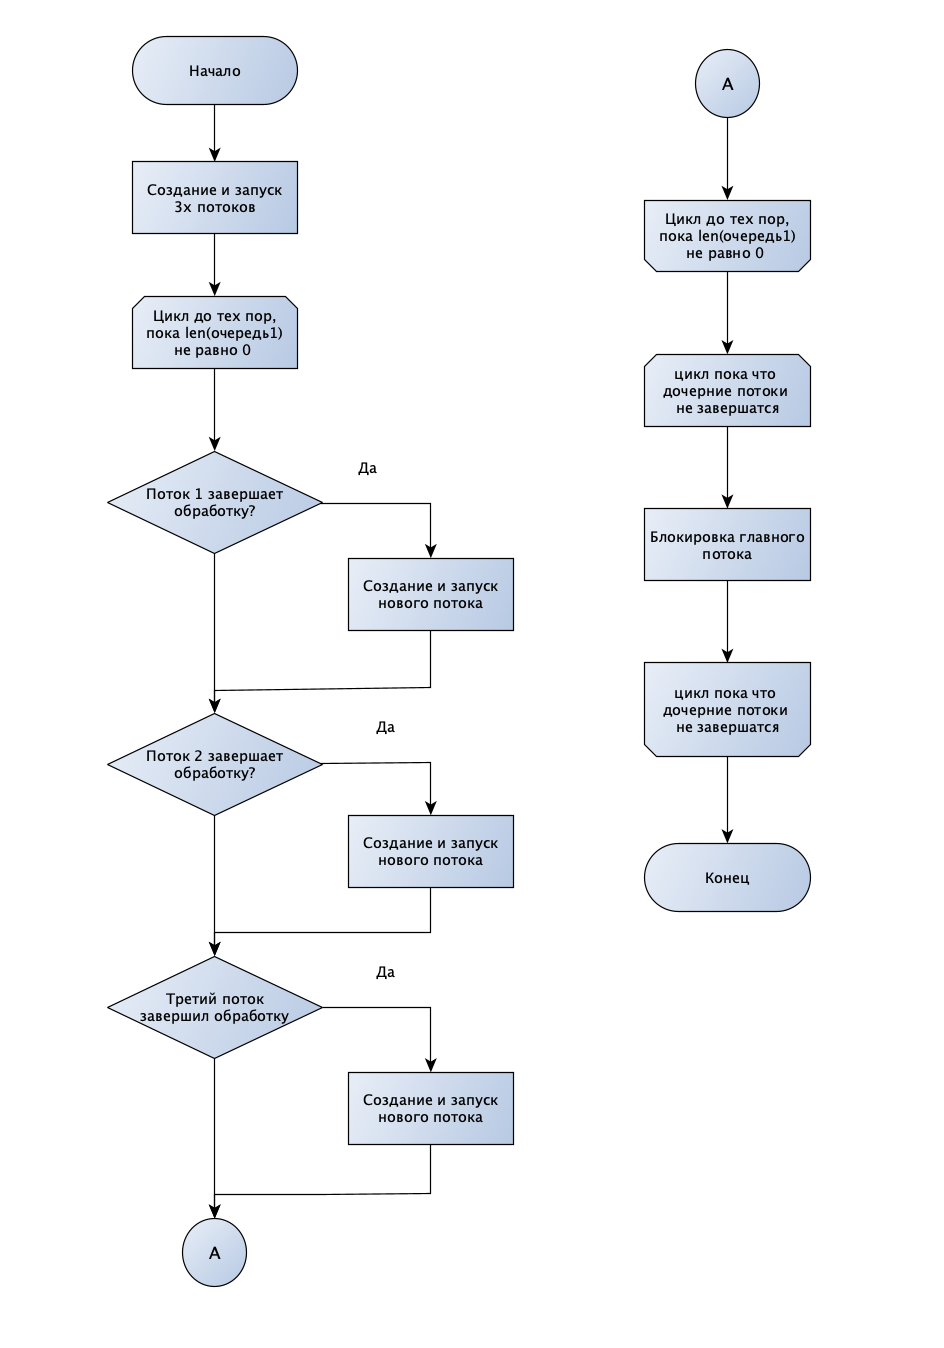
\includegraphics[scale=0.6]{MainThread.png}
		
			Рис 2.1: Схема главного потока
\end{center}

\newpage
\section{Схема рабочего потока}

На рисунке 2.2 представлена схема рабочего потока

\begin{center}
		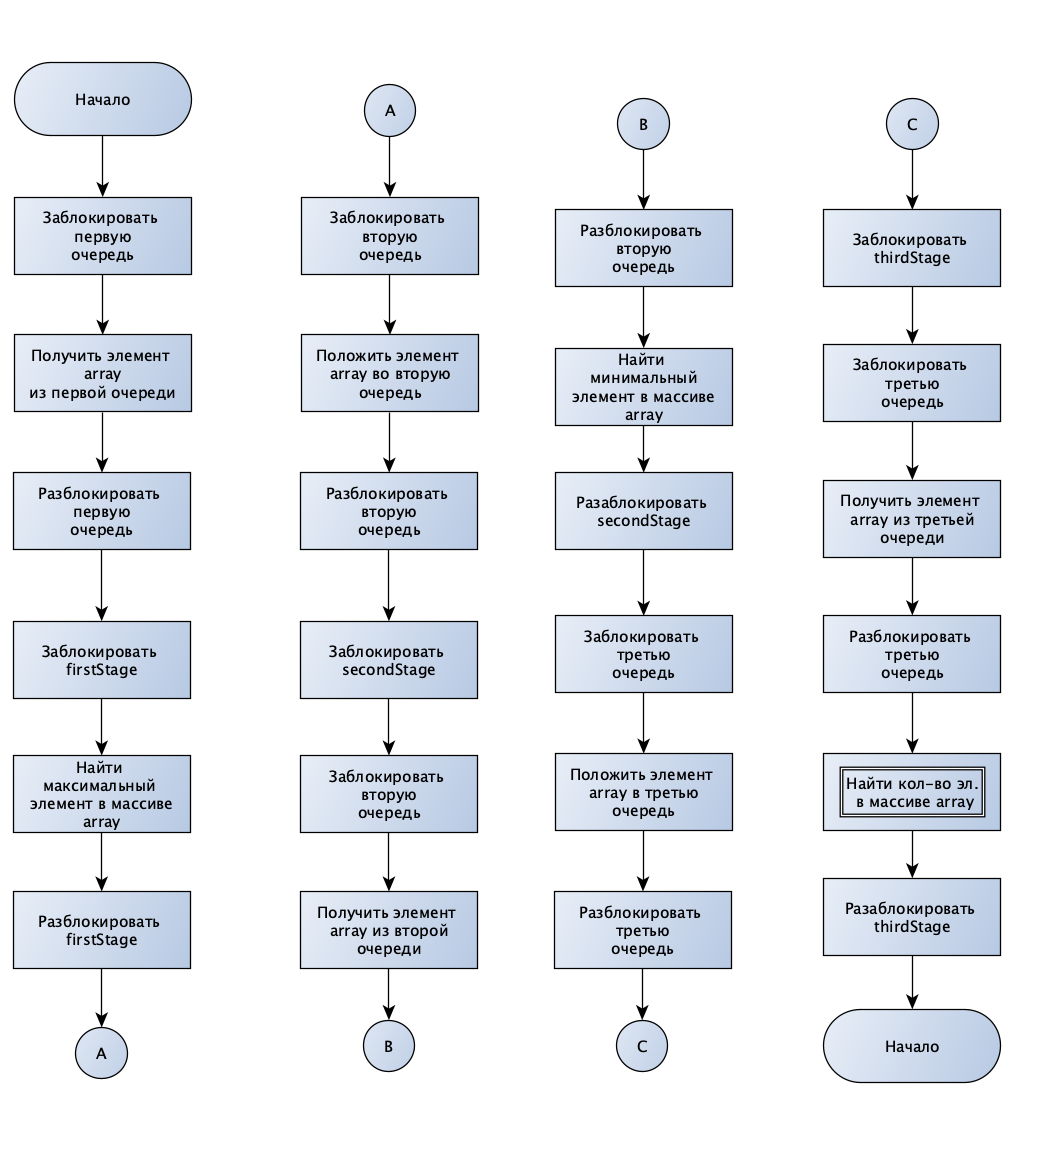
\includegraphics[scale=0.5]{Thread.png}
		
			Рис 2.2: Схема рабочего потока
\end{center}

\section{Вывод}
В данном разделе были рассмотрены 2 схемы: схема главного и рабочего потоков реализации конвейерной обработки данных для решения задачи поиска максимума, минимума и подсчета элементов массива. 

\chapter{Технологическая часть}
\section{Выбор языка программирования}
В данной лабораторной работе использовался язык программирования - С\# \cite{C}, так как данный язык программирования поддерживает параллельное программирования, он является нативным. В качестве интегрированной среды разработки использовалась Visual studio  \cite{Vs}.  Для генерации массива использовался метод Next класса Random \cite{Rand}.

\section{Сведения о модулях программы}
Программа состоит из следующих модулей.
\begin{itemize}
	\item Program.cs - основная программа.
\end{itemize}

На листинге 3.1 представлена подпрограмма главного потока.
\begin{lstlisting}[label=some-code,caption=Метод создания и запуска потоков]
public static void MainTread(Queue<intPtr> queue)
{
	ThreadArgs args = new ThreadArgs(queue);

	Thread firstThread = new Thread(new ParameterizedThreadStart(Conveyor));
	firstThread.Name = "Thread 1";

	Thread secondThread = new Thread(new ParameterizedThreadStart(Conveyor));
	secondThread.Name = "Thread 2";

	Thread thirdThread = new Thread(new ParameterizedThreadStart(Conveyor));
	thirdThread.Name = "Thread 3";

	firstThread.Start(args);
	secondThread.Start(args);
	thirdThread.Start(args);


	while (args.firstQueue.Count != 0)
	{
		if (!firstThread.IsAlive)
		{
			firstThread = new Thread(new ParameterizedThreadStart(Conveyor));
			firstThread.Name = "Thread 1";
			firstThread.Start(args);
		}

		if (!secondThread.IsAlive)
		{
			secondThread = new Thread(new ParameterizedThreadStart(Conveyor));
			secondThread.Name = "Thread 2";
			secondThread.Start(args);
		}

		if (!thirdThread.IsAlive)
		{
			thirdThread = new Thread(new ParameterizedThreadStart(Conveyor));
			thirdThread.Name = "Thread 3";
			thirdThread.Start(args);
		}
	}
}\end{lstlisting}

На листинге 3.2 представлена подпрограмма конвейера.

\begin{lstlisting}[label=some-code,caption=Конвейер]
public static void Conveyor(object obj)
{
	ThreadArgs args = (ThreadArgs)obj;
	int max, min, count;
	intPtr array;

	lock (args.firstQueue)
	{
		// Get array from the first queue.
		array = args.firstQueue.Dequeue();
	}

	lock (firstStage)
	{
		// The first tape is running.
		max = FindMax(array);
	}

	lock (args.secondQueue)
	{
		// Added element to the second queue.
		args.secondQueue.Enqueue(array);
	}

	lock (secondStage)
	{
		// The second tape is running.
		lock (args.secondQueue)
		{
			// Get array from the second queue.
			array = args.secondQueue.Dequeue();
		}
		min = FindMin(array);
	}

	lock (args.thirdQueue)
	{
		args.thirdQueue.Enqueue(array);
	}

	lock (thirdStage)
	{
		lock (args.thirdQueue)
		{
			array = args.thirdQueue.Dequeue();
		}
		count = FindCount(array);
	}
}
\end{lstlisting}

На листинге 3.3 представлена подпрограмма поиска максимума массива.

\begin{lstlisting}[label=some-code,caption=Подпрограмма поиска максимума массива]
public static int FindMax(intPtr array)
{
	int max = array[0];

	for (int i = 0; i < operationsCount; i++)
	foreach (var elem in array)
	if (elem > max)
		max = elem;

	return max;
}
\end{lstlisting}

На листинге 3.4 представлена подпрограмма поиска минимума массива.

\begin{lstlisting}[label=some-code,caption=Подпрограмма поиска минимума массива]
public static int FindMin(intPtr array)
{
	int min = array[0];

	for (int i = 0; i < operationsCount; i++)
	foreach (var elem in array)
	if (elem < min)
		min = elem;

	return min;
}
\end{lstlisting}

На листинге 3.5 представлена подпрограмма поиска количества элементов массива.

\begin{lstlisting}[label=some-code,caption= Подпрограмма поиска количества элементов массива]
public static int FindCount(intPtr array, int num)
{
	int count = 0;

	for (int i = 0; i < operationsCount; i++)
	foreach (var elem in array)
	if (elem < num)
		count++;

	return count;
} 
\end{lstlisting}


\section{Вывод}
В технологической части были представлены модули программы, листинги кода, а также обусловлен выбор языка программирования и приведены использовавшиеся в ходе работы инструменты.

\chapter{Исследовательская часть}

В этом разделе будет проведено сравнение последовательной реализации трех алгоритмов и конвейера с использованием параллельного режима программирования, а также показана статистика.

\section{Характеристики ЭВМ}

\begin{itemize}
	\item MacBook Pro (Retina, 15-inch, Mid 2014).
	\item 2,5 GHz Intel Core i7.
	\item Число логических ядер: 8.
\end{itemize}

\section{Временные характеристики} 

Для сравнения возьмем 10 массивов размерностью
$[$5, 10, 25, 50, 100, 250, 1000$]$.
Воспользуемся усреднением массового эксперимента.

Результат сравнения последовательной реализации трех алгоритмов
при конвейерной обработке данных с использованием параллельной реализации того же алгоритма представлен на рис. \ref{ref:time}.

\begin{figure}[ht!]
	\centering{
		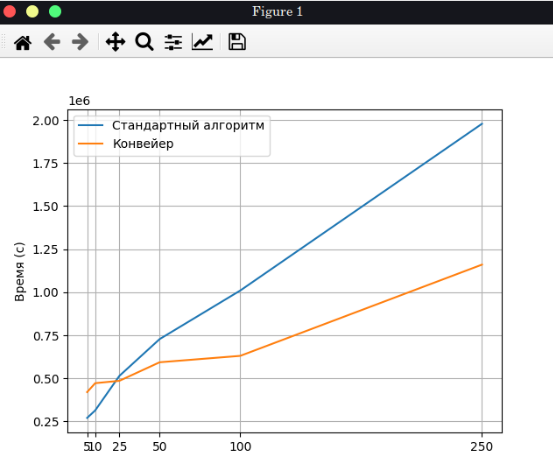
\includegraphics[width=0.8\textwidth]{time.png}
		\caption{Временные характеристики}
		\label{ref:time}}
\end{figure}

По результатам эксперимента видно, что время испольнения конвейерной
реализации значительно меньше, чем исполнение традиционной реализации.
В начале традиционная реализация выигрывает по времени, потому что
при маленьких задачах тратится много времени на создание потоков и
ожидание доступа к переменной, что значительно снижает
работоспособность программы.

На рис. \ref{ref:res} приведена статистика.

\begin{figure}[ht!]
	\centering{
		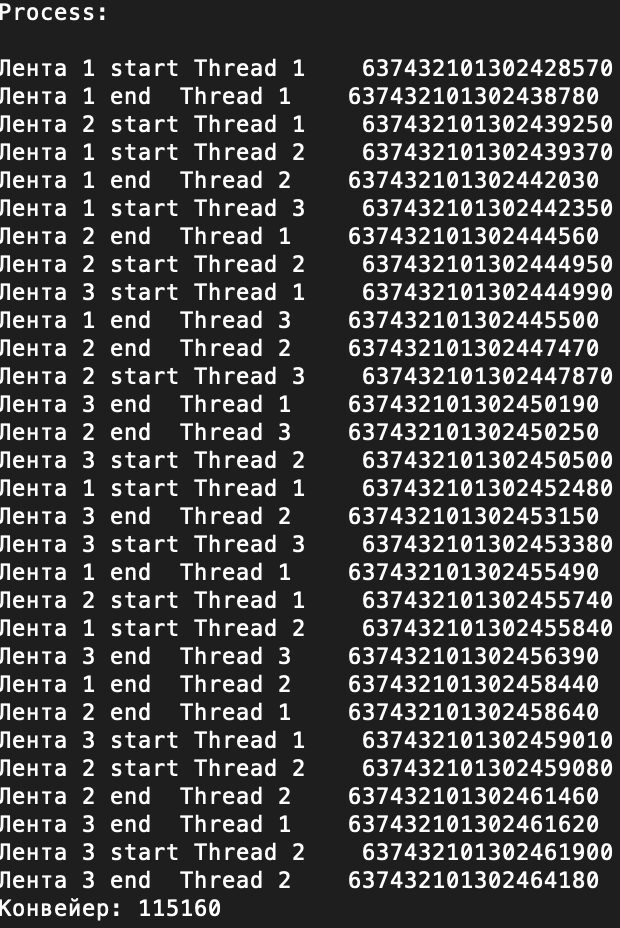
\includegraphics[width=0.6\textwidth]{res.png}
		\caption{Временные характеристики}
		\label{ref:res}}
\end{figure}

\section{Вывод}

В данном разделе было произведено сравнение последовательной реализации трех алгоритмов и конвейера с использованием нескольких потоков. По результатам исследования конвейерную обработку нет смысла применять на задачах, занимающих мало времени. Статистика показала, что конвейерная обработка работает правильно.

\chapter*{Заключение}
\addcontentsline{toc}{chapter}{Заключение}
В ходе лабораторной работы был изучен и реализован конвейер для выполнения элементарных операций на массиве, а также проведен сравнительный анализ затрачиваемых временных ресурсов при параллельной и однопоточной реализаций одного и того же алгоритма. 

В рамках выполнения работы решены следующие задачи.

\begin{enumerate}
\item Изучены основы конвейерной обработки данных.
\item  Получены практические навыки конвейерной обработки данных.
\item Программно реализованы три алгоритма: поиск максимума в массиве, поиск минимума в массиве, поиск количества элементов массива.
\item Сделан сравнительный анализ по затрачиваемым ресурсам (времени) компьютера.
\end{enumerate}

%\bibliographystyle{gost780u}
%\bibliography{books}

\addcontentsline{toc}{chapter}{Список литературы}
\begin{thebibliography}{3}
	\bibitem{Vs}
	Visual Studio [Электронный ресурс], режим доступа:https://visualstudio.microsoft.com/ru/ (дата обращения: 01.10.2020)
	\bibitem{C}
	Документация по C\# [Электронный ресурс], режим доступа:https://docs.microsoft.com/ru-ru/dotnet/csharp/ (дата обращения: 02.10.2020)
	\bibitem{MicrosoftPar}
	Академия Microsoft: Основы параллельного программирования с использованием Visual Studio [Электронный ресурс], - режим доступа: https://intuit.ru/studies/courses/4807/1055/lecture/16369 (дата обращения: 02.10.2020)
	\bibitem{MaxMin}
	 Алгоритм поиска максимума в массиве [Электронный ресурс], режим доступа:https://proglib.io/p/fastest-max-algorithm (дата обращения: 05.12.2020)
	\bibitem{Rand}
	Random Класс [Электронный ресурс], режим доступа:https://docs.microsoft.com/ru-ru/dotnet/api/system.random?view=netcore-3.1 (дата обращения: 02.12.2020)
	 \bibitem{Conveyer}
	Конвейерная организация [Электронный ресурс], режим доступа:https://docs.microsoft.com/ru-ru/dotnet/api/system.random?view=netcore-3.1 (дата обращения: 01.12.2020)
\end{thebibliography}


\end{document}